\documentclass[a4paper,12pt]{article}

\usepackage[top = 2.5cm, bottom = 2.5cm, left = 2.5cm, right = 2.5cm]{geometry}
\usepackage[T1]{fontenc}
\usepackage[utf8]{inputenc}
\usepackage{hyperref}
\usepackage{multirow}
\usepackage{booktabs,amsmath,amsthm}
\usepackage{changepage}
\usepackage{graphicx} 
\usepackage{setspace}
\usepackage{amsthm}
\usepackage{comment}
\usepackage{float}
\usepackage{fancyhdr}
\usepackage{pgfplots}
\usepackage{ulem}

\setlength{\parindent}{0in}
\pagestyle{fancy} 
\fancyhf{}
\pgfplotsset{compat=1.18}

\newtheoremstyle{nonitalic}
  {3pt}
  {3pt}
  {\normalfont}
  {}
  {\bfseries}
  {.}
  {.5em}
  {}

\theoremstyle{nonitalic}

\newtheorem{definition}{Definition}[subsection]

\newtheorem{theorem}{Theorem}[subsection]

\lhead{\footnotesize STA260 Notes}
\rhead{\footnotesize sytez} 
\cfoot{\footnotesize \thepage}

\begin{document}
    \thispagestyle{empty}

    \begin{tabular}{p{15.5cm}}  
        {\Large \bf STA260 Notes}\\
        By sytez\\
        \hline
    \end{tabular}

    \begin{center}
        {\Large \bf Preface}
    \end{center}

    \quad These notes were made for the course STA260: Probability and Statistics II at the University of Toronto Mississauga. They are based on the lectures and lecture slides of the 2024 summer offering. This course was instructed by Professor Luai Al Labadi (The Goat). These notes primarily consist of a summary of the defintions and theorems from the course. The notes are not exhaustive and may contain errors. The proofs provided are not complete and instead provide a brief outline of the proof containing the main ideas. Theorems that do not contain a proof are usually trivial to prove with exceptions of the ones whose proof is beyond the scope of this course.

    \newpage
    
    \tableofcontents
    \newpage

    \setcounter{section}{6}

    \section{Chapter 7 \textemdash{} Sampling Distributions and the Central Limit Theorem}

    \subsection{Introduction}

    \begin{definition}
        A \textbf{population} consists of the entire collection of the observations with which we are concerned.
    \end{definition}

    \bigskip

    \begin{definition}
        A \textbf{sample} is a subset of a population.
    \end{definition}

    \bigskip

    \begin{definition}
        A \textbf{parameter} is a numerical summary of a population. For example, the mean, the variance, etc. In practice, it is unknown.
    \end{definition}

    \bigskip

    \begin{definition}
        A \textbf{statistic} is a numerical summary of a sample. For example, the sample mean, the sample variance, etc.
    \end{definition}

    \bigskip

    \begin{definition}
        The statistic varies from sample to sample and hence it is a random variable and has a probability distribution called the \textbf{sampling distribution}.
    \end{definition}

    \bigskip

    The knowledge of the sampling distribution of a statistic helps to make an inference about the corresponding population (true) parameter.

    \bigskip

    \begin{definition}
        We say that the random variables $Y_1, Y_2, \ldots, Y_n$ are \textbf{independent and identically distributed} (i.i.d.) if they are independent random variables and have the same probability distribution (same pdf/cdf).
    \end{definition}

    \bigskip

    For a random sample, we write
    \[
        Y_1, \ldots, Y_n \overset{\text{i.i.d.}}{\sim} f(y) \quad \text{(continuous)}
    \]
    \[
        Y_1, \ldots, Y_n \overset{\text{i.i.d.}}{\sim} p(y) \quad \text{(discrete)}
    \]
    \newpage

    \subsection{Sampling Distributions}
    
    \begin{definition}
        The \textbf{sample mean} is defined as
        \[
            \overline{Y} = \frac{1}{n} \sum_{i=1}^{n} Y_i
        \]
    \end{definition}

    \begin{definition}
        The \textbf{sample variance} is defined as
        \[
            S^2 = \frac{1}{n-1} \sum_{i=1}^{n} (Y_i - \overline{Y})^2
        \]
    \end{definition}

    \begin{theorem}
        Let $Y_1, \ldots, Y_n$ be an iid random sample from a population with any distribution with finite mean $\mu$ and finite variance $\sigma^2$. Then \(E(\overline{Y}) = \mu\) and \(V(\overline{Y}) = \frac{\sigma^2}{n}\).
    \end{theorem}

    \begin{theorem}
        If $Y_1, \ldots, Y_n \overset{\text{i.i.d.}}{\sim} N\left(\mu, \sigma^2\right)$, then
        \[
        \overline{Y} \sim N\left(\mu, \frac{\sigma^2}{n}\right)
        \]
    \end{theorem}
    
    
    \begin{proof}
        Show MGF of $\overline{Y}$ is the MGF of $N\left(\mu, \frac{\sigma^2}{n}\right)$ then conclude by uniqueness of MGF.
    \end{proof}
    
    \begin{definition}
        The \textbf{standard normal distribution} is defined as
        \[
            Z = \frac{Y - \mu}{\sigma} = \frac{\overline{Y} - \mu}{\sigma/\sqrt{n}} = N(0,1)
        \]
    \end{definition}

    \begin{theorem}
        Let \( Y_1, \ldots, Y_n \overset{\text{i.i.d.}}{\sim} N(\mu, \sigma^2) \). If \( Z_i = \frac{Y_i - \mu}{\sigma} \), then
        \[
        \sum_{i=1}^{n} Z_i^2 = \sum_{i=1}^{n} \left( \frac{Y_i - \mu}{\sigma} \right)^2
        \]
        has a \(\chi^2\) distribution with \(n\) degrees of freedom (df)
    \end{theorem}
    
    \begin{proof}
        Note 3 facts:
        \begin{enumerate}
            \item \(\chi^2_{(v)} = \text{Gamma}(v/2, 2)\)
            \item \(\chi^2_{(v_1)} + \chi^2_{(v_2)} \sim \chi^2_{(v_1 + v_2)}\) assuming independence
            \item \([N(0,1)]^2 = Z^2 \sim \chi^2_{(1)}\)
        \end{enumerate}

        The proof becomes trivial from here.
    \end{proof}

    Note that similarly we have the sum of many distributions can be studied easily.
    \[\begin{aligned}
        &Y_1, \ldots, Y_n \overset{\text{iid}}{\sim} \text{Ber}(p) \implies \sum_{i=1}^{n} Y_i \sim \text{Bin}(n, p) \\
        &Y_1, \ldots, Y_n \overset{\text{iid}}{\sim} \text{Poisson}(\lambda) \implies \sum_{i=1}^{n} Y_i \sim \text{Poisson}(n\lambda) \\
        &Y_1, \ldots, Y_n \overset{\text{iid}}{\sim} \chi^2(v_i) \implies \sum_{i=1}^{n} Y_i \sim \chi^2_{\left(\sum\limits_{i=1}^{n} v_i\right)}\\
        &Y_1, \ldots, Y_n \overset{\text{iid}}{\sim} N(\mu_i, \sigma^2_i) \implies \sum_{i=1}^{n} Y_i \sim N\left(\sum\limits_{i=1}^{n} \mu_i, \sum\limits_{i=1}^{n} \sigma^2_i\right)
    \end{aligned}\]

    \begin{proof}
        Note the following fact:\\
        Let $U = Y_1 + \ldots + Y_n$ then we have $M_U(t) = M_{Y_1}(t) \cdot \ldots \cdot M_{Y_n}(t)$.\\
        That is that the MGF of the sum of random variables is the product of the MGFs of the random variables.\\
        The proof follows trivially using the unqiueness of MGFs.
    \end{proof}

    \begin{theorem}
        As a corollary of theorem 7.2.2\\
        If \( Y_1, \ldots, Y_n \overset{\text{i.i.d.}}{\sim} N(\mu, \sigma^2) \), then
        \[
            U = \sum_{i=1}^{n} \left( \frac{Y_i - \mu}{\sigma} \right)^2 \sim \chi^2_{(n)}
        \]
        similarly one sees that if \( Y_i \sim N(\mu_i, \sigma_i^2), \, i = 1, \ldots, n \) (and independent), then
        \[
        U = \sum_{i=1}^{n} \left( \frac{Y_i - \mu_i}{\sigma_i} \right)^2 \sim \chi^2(n).
        \]
    \end{theorem}

    \begin{theorem}
        Let \( Y_1, Y_2, \ldots, Y_n \) be a random sample from a normal distribution with mean \(\mu\) and variance \(\sigma^2\). Then
        \[
        \frac{(n-1)S^2}{\sigma^2} = \sum_{i=1}^{n} \frac{(Y_i - \overline{Y})^2}{\sigma^2} \sim \chi^2_{n-1}.
        \]
        Additionally, \(\overline{Y}\) and \(S^2\) are independent.
    \end{theorem}

    \newpage

    \subsection{The t-Distribution}

    \begin{definition}
        Let $Z \sim N(0,1)$ and $W \sim \chi^2_{(v)}$. Then if $Z$ and $W$ are independent then we say
        \[
            T = \frac{Z}{\sqrt{W/v}} \sim t_{(v)}
        \]
        has a \textbf{$t$-Distribution} with $v$ degrees of freedom.
    \end{definition}

    So far it was assumed that the population standard deviation $\sigma$ is known. However, this assumption may be unreasonable. We want to estimate both $\mu$ and $\sigma$. A natural statistic to deal with inferences on $\mu$ is
    \[
        T = \frac{\overline{Y} - \mu}{S/\sqrt{n}} \sim t_{(n-1)}
    \]
    
    \textbf{Properties of the $t$-Distribution}
    
    \begin{figure}[h!]
        \centering
        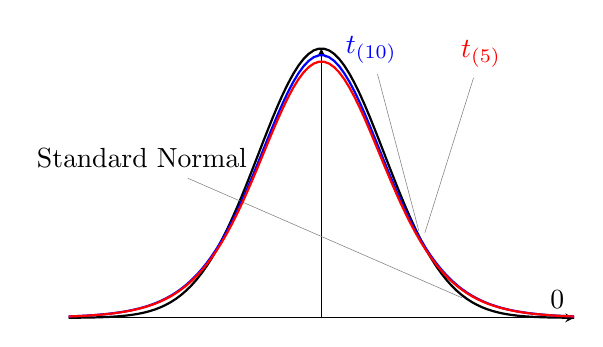
\begin{tikzpicture}
            \begin{axis}[
                axis lines=middle,
                xlabel={$0$},
                ylabel={},
                xtick=\empty,
                ytick=\empty,
                ymin=0,
                xmin=-4, xmax=4,
                samples=100,
                height=5cm,
                width=8cm,
                enlarge x limits=false,
                enlarge y limits=false,
                clip=false,
                ]
                % Standard Normal Curve
                \addplot[thick, black, domain=-4:4] {1/sqrt(2*pi) * exp(-0.5*x^2)} node[pos=0.8, pin={[pin distance=3cm]150:Standard Normal}] {};
                % t-distribution Curve (with 10 degrees of freedom)
                % (gamma(11/2)/(sqrt(10*pi)*gamma(5))) = 0.389108383
                \addplot[thick, blue, domain=-4:4] {0.389108383 * (1 + x^2/10)^(-11/2)} node[pos=0.7, pin={[pin distance=2cm]95:$t_{(10)}$}] {};
                % t-distribution Curve (with 5 degrees of freedom)
                % (gamma(3)/(sqrt(5*pi)*gamma(5/2))) = 0.379606689
                \addplot[thick, red, domain=-4:4] {0.379606689 * (1 + x^2/10)^(-11/2)} node[pos=0.7, pin={[pin distance=2cm]80:$t_{(5)}$}] {};
            \end{axis}
        \end{tikzpicture}
        \caption{Comparison of Standard Normal and $t$-distribution curves with 5 and 10 degrees of freedom}
    \end{figure}

    \begin{itemize}
        \item Each $t_\nu$ curve is bell-shaped and centered at 0.
        \item Each $t_\nu$ curve is spread out more than the standard normal ($Z$) curve.
        \item As $\nu$ increases, the spread of the corresponding $t_\nu$ curve decreases.
        \item As $\nu \to \infty$, the sequence of $t_\nu$ curves approaches the standard normal curve (the $Z$ curve is called a $t$ curve with df $=\infty$).
    \end{itemize}

    \newpage

    \subsection{The F-Distribution}

    \begin{definition}
        Let \( W_1 \sim \chi^2_{(\nu_1)} \) and \( W_2 \sim \chi^2_{(\nu_2)} \) be independent. Then
        \[
            F = \frac{W_1 / \nu_1}{W_2 / \nu_2}
        \]
        has a \textbf{\( F \)-Distribution} with \( \nu_1 \) and \( \nu_2 \) degrees of freedom.
    \end{definition}

    \begin{theorem}
        If \( S_1^2 \) and \( S_2^2 \) are the variances of independent random samples of size \( n_1 \) and \( n_2 \) taken from normal populations with variances \( \sigma_1^2 \) and \( \sigma_2^2 \), respectively, then
        \[
        \frac{S_1^2 / \sigma_1^2}{S_2^2 / \sigma_2^2} \sim F(n_1 - 1, n_2 - 1).
        \]        
    \end{theorem}

    \begin{proof}
        Recall that
        \[
            \frac{(n-1)S^2}{\sigma^2} \sim \chi^2_{(n-1)}
        \]
        the proof trivially follows.
    \end{proof}
    
    \begin{theorem}
        Let $Y$ be a random variable such that $Y \sim F_{(v_1, v_2)}$. Then
        \[
            \frac{1}{Y} \sim F_{(v_2, v_1)}
        \]
    \end{theorem}

    \begin{theorem}
        Let $Y_1 \sim F_{(v_1, v_2)}$ then
        \[
            \left(1 + \frac{v_1}{v_2}Y_1\right)^{-1} \sim \text{Beta}\left(\frac{v_2}{2}, \frac{v_1}{2}\right)
        \]
    \end{theorem}
    
    \begin{proof}
        Recall that
        \[
            \chi^2_{(v)} = \text{Gamma}\left(\frac{v}{2}, 2\right) \quad \text{and} \quad \frac{\text{Gamma}(\alpha, \gamma)}{\text{Gamma}(\alpha, \gamma) + \text{Gamma}(\beta, \gamma)} = \text{Beta}(\alpha, \beta)
        \]
        the proof follows trivially using the defintion of the $F$-distribution.
    \end{proof}

    \begin{theorem}
        Let $T$ be a random variable with a $t$-distribution with $v$ degrees of freedom. Then $U = T^2$ has an $F$-distribution with $1$ and $v$ degrees of freedom.
    \end{theorem}

    \newpage

    \subsection{The Central Limit Theorem}

    We already showed that if \(Y_1, Y_2, \ldots, Y_n\) represents a random sample from any distribution with mean \(\mu\) and variance \(\sigma^2\), then \(E(\overline{Y}) = \mu\) and \(V(\overline{Y}) = \frac{\sigma^2}{n}\).\\
    In what follows, we will develop an approximation for the sampling distribution of \(\overline{Y}\) that can be used \uline{regardless of the distribution of the population from which the sample is taken}.

    \bigskip

    \begin{theorem} \textbf{Central Limit Theorem}\\
        Let \(Y_1, Y_2, \cdots, Y_n\) be a random sample from a population with finite mean \(\mu\) and finite variance \(\sigma^2\), but unknown distribution. Then if \(n\) is sufficiently large, \(\overline{Y}\) is \textcolor{red}{approximately normally distributed} with mean \(\mu\) and variance \(\frac{\sigma^2}{n}\), i.e. $\overline{Y} \approx N(\mu, \frac{\sigma^2}{n})$.
    \end{theorem}

    \bigskip

    The CLT can be written more formally as:\\
    If
    \[
        U_n = \frac{\sum_{i=1}^n Y_i - n\mu}{\sigma \sqrt{n}} = \frac{\overline{Y} - \mu}{\sigma / \sqrt{n}}
    \]
    then
    \[
        U_n \overset{d}{\to} N(0, 1)
    \]

    This implies that
    \[
        \lim_{n \to \infty} P(U_n \leq u) = \int_{-\infty}^{u} \frac{1}{\sqrt{2\pi}} e^{-t^2/2} \, dt
    \]

    \begin{proof}
        Let $U_n = \frac{\overline{Y} - \mu}{\sigma / \sqrt{n}}$, now we can rewrite $U_n = \frac{1}{\sqrt{n}} \sum\limits_{i=1}^{n} Z_i$.\\
        Now note that
        \[
            M_{U_n}(t) = M_{\frac{1}{\sqrt{n}} \sum\limits_{i=1}^{n} Z_i}(t) = M_{\sum\limits_{i=1}^{n} Z_i}\left(\frac{t}{\sqrt n}\right) = \prod_{i=1}^{n} M_{Z_i} \left(\frac{t}{\sqrt n}\right) = \left[M_{Z_1}\left(\frac{t}{\sqrt{n}}\right)\right]^n
        \]
        Now through the use of the McLaurin expansion of \(M_{Z_1}\left(\frac{t}{\sqrt{n}}\right)\) it can be shown that
        \[
            \lim_{n \to \infty} n \cdot M_{Z_1}\left(\frac{t}{\sqrt{n}}\right) - n = \frac{t^2}{2}
        \]

        Now note that
        \[
            \lim_{n \to \infty} b_n = b \implies \lim_{n \to \infty} \left(1 + \frac{b_n}{n}\right)^n = e^b
        \]

        Thus we see that
        \[
            \lim_{n \to \infty} M_{U_n}(t) = \lim_{n \to \infty} \left[M_{Z_1}\left(\frac{t}{\sqrt{n}}\right)\right]^n = e^{\frac{t^2}{2}}
        \]

        Thus we see that $\lim\limits_{n \to \infty} M_{U_n}(t) = M_{N(0,1)}(t)$ and thus by the uniqueness of MGFs we see that $U_n \overset{d}{\to} N(0,1)$.
    \end{proof}

    \bigskip

    The \textbf{Central Limit Theorem} states that the sample mean from any probability distribution (as long as mean and variance are \uline{finite}) will have an approximate normal distribution, if the sample is sufficiently large.

    \bigskip

    ``Large \( n \)'' means \( n \geq 30 \) in general, but in some cases may even be much less.

    \bigskip

    The larger the sample size, the more nearly normally distributed is the population of all possible sample means.

    \bigskip

    For fairly symmetric distributions, \( n > 15 \) will be sufficient.

    \newpage

    \subsection{Normal Approximation to the Binomial}

    The normal distribution (continuous) can be used to approximate binomial (discrete) probabilities when there is a very large number of trials and when \(np\) and \(n(1 - p)\) are both large (\(np \geq 5\) and \(n(1 - p) \geq 5\)).

    \bigskip

    \begin{theorem}
        \textbf{Normal Approximation to the Binomial}\\
        If \(Y \sim \text{Bin}(n,p)\), then \(Y \approx N(\mu = np, \sigma^2 = npq)\)
    \end{theorem}

    \begin{proof}
        The justification for the normal approximation to the binomial is based on the Central Limit Theorem.
    \end{proof}

    \bigskip
    
    To improve the accuracy of the approximation, we usually use a correction factor, \uline{called continuity correction}, to take into account that the binomial random variable is discrete while the normal is continuous.

    \bigskip

    The basic idea is to treat the discrete value \(b\) as the continuous interval from \(b - 0.5\) to \(b + 0.5\) giving the following adjustments:

    \begin{itemize}
        \item \(P(Y = b) = P(b - 0.5 \leq Y \leq b + 0.5)\)
        \item \(P(Y \leq b) = P(Y \leq b + 0.5)\)
        \item \(P(b \leq Y) = P(b - 0.5 \leq Y)\)
    \end{itemize}

    \newpage

    \section{Chapter 8 \textemdash{} Estimation}

    If \( Y_1, Y_2, \ldots, Y_n \overset{i.i.d.}{\sim} N(\mu, 1) \), where \(\mu\) is unknown, then how do we estimate \(\mu\)?
    
    \bigskip

    An \textcolor{red}{estimator} is a rule, often expressed as a formula, that tells how to calculate the value of an estimate based on the measurements contained in a sample.
    
    \bigskip

    Let \( Y_1, Y_2, \ldots, Y_n \) be i.i.d. with pdf/pmf \( f = f(\cdot|\theta) = f_\theta \), where the parameter \(\theta\) is unknown ($f$ depends on $\theta$). We want to find an estimate for the unknown parameter \(\theta\).

    \subsection{Point Estimation}
    \begin{definition}
        A \textbf{point estimator} $\hat{\theta}$ of the parameter \(\theta\) is a function of the underlying random variables and so it is a random variable with a distribution function.
    \end{definition}

    \bigskip

    A point estimate of \(\theta\) is a function of the sample \(Y_1, Y_2, \ldots, Y_n\) only. That is if $y_1, \ldots, y_n$ is the observed sample then $\hat{\theta} = U(y_1, \ldots, y_n)$ is a number.

    \bigskip

    For example a distribution with mean $\mu$ and variance $\sigma^2$ we have that $\overline{Y}$ is a point estimator for $\mu$ and $S^2$ is a point estimator for $\sigma^2$.

    \bigskip

    We say that a point estimator $\hat{\theta}$ is "good" if it has the following desirable properties:
    \begin{enumerate}
        \item Unbiased
        \item Consistent
        \item Minimum Variance
        \item Has a known probability distribution
    \end{enumerate}
    
    \begin{definition}
        Let $\hat{\theta}$ be a point estimator for a parameter $\theta$. Then $\hat{\theta}$ is an \textbf{unbiased estimator} if $E(\hat{\theta}) = \theta$. If $E(\hat{\theta}) \neq \theta$, then $\hat{\theta}$ is said to be \textbf{biased}.
    \end{definition}
    Note that $\hat{\theta}$ is a random variable whereas $\theta$ is a constant.

    \bigskip

    \begin{definition}
        The \textbf{bias} of a point estimator $\hat{\theta}$ is given by $B(\hat{\theta}) = E(\hat{\theta}) - \theta$.
    \end{definition}
    We see that a point estimator $\hat{\theta}$ is unbiased w.r.t. $\theta$ if $B(\hat{\theta}) = 0$.

    \bigskip
        
    \begin{definition}
        The \textbf{mean square error} of a point estimator $\hat{\theta}$ is $MSE(\hat{\theta}) = E\left[ (\hat{\theta} - \theta)^2 \right]$.
    \end{definition}

    \begin{theorem}
        $MSE(\hat{\theta}) = V(\hat{\theta}) + \left[B(\hat{\theta})\right]^2$
    \end{theorem}
    It can be seen that if the estimator is unbiased then $MSE(\hat{\theta}) = V(\hat{\theta})$.

    \bigskip

    \textbf{Examples of Well-Known Unbiased Estimators}

    Let $Y_1, Y_2, \ldots, Y_n$ be a random sample with $E(Y_i) = \mu_1$ and $X_1, X_2, \ldots, X_n$ be a random sample with $E(X_i) = \mu_2$. Then:

    \begin{align*}
        E\left(\overline{Y}\right) &= \mu_1 \quad \text{and} \quad E\left(\overline{X}\right) = \mu_2\\
        E\left(\overline{Y} - \overline{X}\right) &= \mu_1 - \mu_2
    \end{align*}
    
    Let $Y \sim \text{Bin}(n, p_1)$ and $X \sim \text{Bin}(n, p_2)$. Then $\hat{p}_1 = \frac{Y}{n}$ is the proportion of successes in the sample.
    
    \begin{align*}
        E\left(\hat{p}_1\right) &= E\left(\frac{Y}{n}\right) = \frac{1}{n} E(Y) = \frac{np_1}{n} = p_1\\
        E\left(\hat{p}_2\right) &= E\left(\frac{X}{n}\right) = \frac{1}{n} E(X) = \frac{np_2}{n} = p_2\\
        E\left(\hat{p}_1 - \hat{p}_2\right) &= p_1 - p_2
    \end{align*}

    \newpage

    \subsection{Evaluating the Goodness of an Estimator}

    \begin{definition}
        Let \(\sigma^2_{\hat{\theta}}\) be the variance of the sampling distribution of the estimator \(\hat{\theta}\)

        (i.e. \(V(\hat{\theta}) = \sigma^2_{\hat{\theta}}\)), then \(\sqrt{V(\hat{\theta})} = \sqrt{\sigma^2_{\hat{\theta}}} = \sigma_{\hat{\theta}}\) is called the \textbf{standard error} of the estimator. That is, the \textbf{standard error} of \(\hat{\theta} =\) the standard deviation of \(\hat{\theta}\).
    \end{definition}
    Note that we call it the standard error because it comes from the sampling process.

    \bigskip

    \begin{definition}
        The \textbf{error of estimation} \(\varepsilon\) is the distance between an estimator and its target parameter. That is, \(\varepsilon = |\hat{\theta} - \theta|\).
    \end{definition}

    \bigskip

    \begin{definition}
        The \textbf{2-standard-error bound} on the error of estimation is given by $2SE(\hat{\theta}) = 2\sigma_{\hat{\theta}}$.
    \end{definition}
    To place a 2-standard-error bound on the error of estimation is to find the probability that the error of estimation is within 2 standard errors of the estimator. That is to find $P(|\varepsilon| < 2SE(\hat{\theta})) = P(|\varepsilon| < 2 \sigma_{\hat{\theta}})$.

    \newpage

    \subsection{Confidence Intervals}

    An alternative to reporting a single value for the parameter being estimated is to calculate and report an entire interval of plausible values; i.e., a \textbf{confidence interval} (CI).

\end{document}